\textbf{Pour cette première partie, aucune justification n'est demandée et une seule réponse est possible par question. Pour chaque question, reportez son numéro sur votre copie et indiquez votre réponse.}

	Une réponse fausse ou l'absence de réponse n'enlève aucun point.

	\subsection*{Question 1}

	On considère la fonction $f$ définie sur $[-5 ; 4]$ représentée dans le repère ci-dessous :

	\begin{center}
		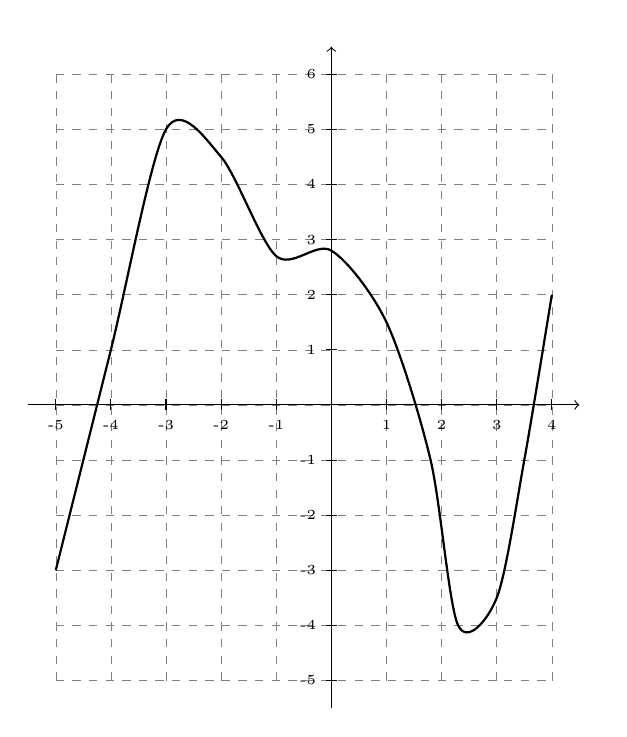
\begin{tikzpicture}[scale=0.7]
			\draw[step=1cm,gray,very thin,dashed] (-5,-5) grid (4,6);
			\draw[->] (-5.5,0) -- (4.5,0) node[right] {};
			\draw[->] (0,-5.5) -- (0,6.5) node[above] {};
			\foreach \x in {-5,-4,-3,-2,-1,1,2,3,4} \draw (\x,0.1) -- (\x,-0.1) node[below] {\tiny \x};
			\foreach \y in {-5,-4,-3,-2,-1,1,2,3,4,5,6} \draw (0.1,\y) -- (-0.1,\y) node[left] {\tiny \y};
			\draw[thick] plot[smooth] coordinates {(-5,-3) (-4,1) (-3,5) (-2,4.5) (-1,2.7) (0,2.8) (1,1.5) (1.8,-1) (2.3,-4) (3,-3.5) (3.5,-1) (4,2)};
		\end{tikzpicture}
	\end{center}

	Sur $[-5 ; 4]$, l'équation $f(x)=-1$ admet :

	\medskip
	\begin{tblr}{colspec = {@{}*{4}{X}}}
		\textbf{A.}\quad zéro solution.&
		\textbf{B.}\quad une seule solution. &
		\textbf{C.}\quad deux solutions. &
		\textbf{D.}\quad trois solutions. \\
	\end{tblr}

	\subsection*{Question 2}

	Multiplier un nombre par 0,6 revient à le diminuer de :

	\medskip
	\begin{tblr}{colspec = {@{}*{4}{X}}}
		\textbf{A.}\quad 4\,\% &
		\textbf{B.}\quad 6\,\% &
		\textbf{C.}\quad 40\,\% &
		\textbf{D.}\quad 60\,\% \\
	\end{tblr}

	\subsection*{Question 3}

	L'équation réduite de la droite représentée dans le repère ci-dessous est :

	\begin{center}
		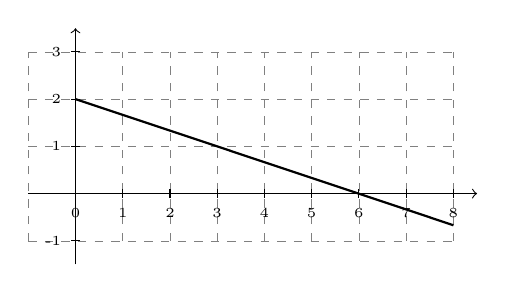
\begin{tikzpicture}[scale=0.6]
			\draw[step=1cm,gray,very thin,dashed] (-1,-1) grid (8,3);
			\draw[->] (-1,0) -- (8.5,0);
			\draw[->] (0,-1.5) -- (0,3.5);
			\foreach \x in {0,1,2,3,4,5,6,7,8} \draw (\x,0.1) -- (\x,-0.1) node[below] {\tiny \x};
			\foreach \y in {-1,1,2,3} \draw (0.1,\y) -- (-0.1,\y) node[left] {\tiny \y};
			\draw[thick] (0,2) -- (8,-0.67);
		\end{tikzpicture}
	\end{center}

	\medskip
	\begin{tblr}{colspec = {@{}*{4}{X}}}
		\textbf{A.}\quad $y=-2x+6$ &
		\textbf{B.}\quad $y = 6x + 2$ &
		\textbf{C.}\quad $y = -\dfrac{1}{3}x + 2$ &
		\textbf{D.}\quad $y = -3x + 2$\\
	\end{tblr}

	\subsection*{Question 4}

	Un club de sport possède 200 adhérents répartis comme l'indique le tableau ci-dessous :

	\begin{center}
		\begin{tblr}{colspec={|X[c,2cm]|X[c,3cm]|X[c,3cm]|X[c,2cm]|}}
			\hline
			& Volley-ball & Basket-ball & Total \\
			\hline
			Enfant & 80 & 50 & 130 \\
			\hline
			Adulte & 30 & 40 & 70 \\
			\hline
			Total & 110 & 90 & 200 \\
			\hline
		\end{tblr}
	\end{center}

	On choisit au hasard un adhérent du club.

	On note les évènements suivants :
	\begin{itemize}[noitemsep,label={}]
		\item $E$ : \og La personne choisie est un enfant. \fg
		\item $V$ : \og La personne choisie pratique le volley-ball. \fg
	\end{itemize}

	On note $P_E(V)$ la probabilité que la personne choisie pratique le volley-ball sachant que c'est un enfant.

	La probabilité $P_E(V)$ est égale à :
	\medskip

	\begin{tblr}{colspec = {@{}*{4}{X}}}
		\textbf{A.}\quad $\dfrac{8}{13}$ &
		\textbf{B.}\quad $\dfrac{8}{11}$ &
		\textbf{C.}\quad $\dfrac{8}{20}$ &
		\textbf{D.}\quad $\dfrac{11}{13}$ \\
	\end{tblr}

	\medskip
	\begin{minipage}[t]{0.5\linewidth}
	\subsection*{Question 5}

	Soient $A$ et $B$ deux évènements.

	En s'appuyant sur l'arbre pondéré ci-dessous, calculer $P(B)$.
	\end{minipage}
	\hfill
	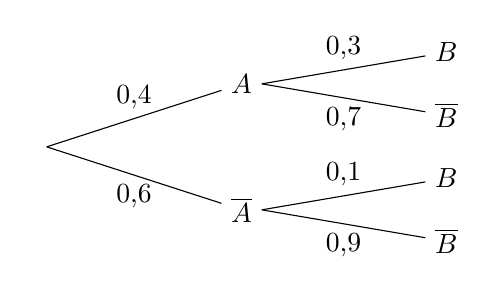
\begin{tikzpicture}[x=2.6cm, y=0.8cm,baseline={(B1.base)}]
		
		\node (root) at (0,0) {};
		\node (A) at (1,1) {$A$};
		\node (Abar) at (1,-1) {$\overline{A}$};
		\node (B1) at (2,1.5) {$B$};
		\node (B1b) at (2,0.5) {$\overline{B}$};
		\node (B2) at (2,-0.5) {$B$};
		\node (B2b) at (2,-1.5) {$\overline{B}$};
		
		\draw (root.east) -- (A) node[pos=0.5,above] {0,4};
		\draw (root.east) -- (Abar) node[pos=0.5,below] {0,6};
		
		\draw (A.east) -- (B1) node[pos=0.5,above] {0,3};
		\draw (A.east) -- (B1b) node[pos=0.5,below] {0,7};
		\draw (Abar.east) -- (B2) node[pos=0.5,above] {0,1};
		\draw (Abar.east) -- (B2b) node[pos=0.5,below] {0,9};
	\end{tikzpicture}
	\hfill~

	\medskip
	\begin{tblr}{colspec = {@{}*{4}{X}}}
		\textbf{A.}\quad 0,4 &
		\textbf{B.}\quad 0,18 &
		\textbf{C.}\quad 0,72 &
		\textbf{D.}\quad 0,03 \\
	\end{tblr}

	\subsection*{Question 6}

	\begin{minipage}[t]{0.5\linewidth}
	On a représenté une fonction affine $f$ et une fonction polynôme du second degré $g$ définies sur $\mathbb{R}$.

	\medskip

	L'ensemble $S$ des solutions de l'inéquation
	\[f(x) < g(x)\]
	est :

	\medskip

	\begin{tblr}{colspec = {@{}*{1}{X}}}
		\textbf{A.}\quad $S=\,]-2 ; 2[$ \\
		\textbf{B.}\quad $S=\,]-\infty ; -2[\,\cup\,]2 ; +\infty[$ \\
		\textbf{C.}\quad $S=\,]-1 ; 0,5[\,\cup\,]3 ; +\infty[$ \\
		\textbf{D.}\quad $S=\,]-1 ; 3[$ \\
	\end{tblr}
	\end{minipage}
	\hfill
	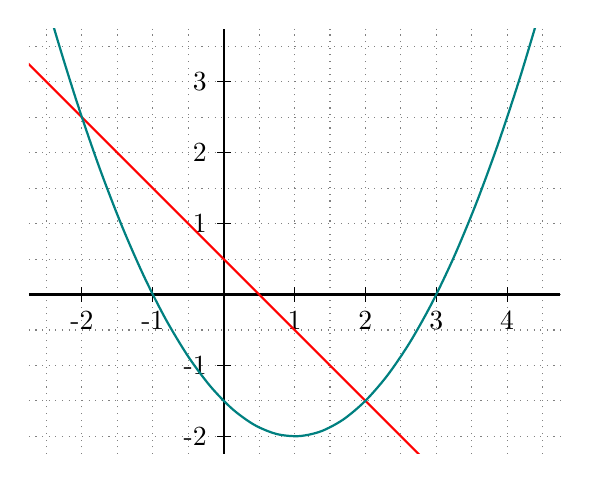
\begin{tikzpicture}[scale=0.9,baseline={(current bounding box.north)}]
		\draw[step=0.5cm,gray,thin,dotted] (-2.75,-2.25) grid (4.75,3.75);
		\draw[line width = .8pt] (-2.75,0) -- (4.75,0)
			(0,-2.25) -- (0,3.75);
		\foreach \x in {-2,-1,1,2,3,4} \draw (\x,0.1) -- (\x,-0.1) node[below] {\np{\x}};
		\foreach \y in {-2,-1,1,2,3} \draw (0.1,\y) -- (-0.1,\y) node[left] {\np{\y}};
		\clip (-2.75,-2.25) rectangle (4.75,3.75);
		\draw[thick,red] (-3,3.5) -- (3,-2.5);
		\draw[thick,teal] plot[smooth,domain=-3:4.5] (\x,{0.5*(\x-1)*(\x-1)-2});
	\end{tikzpicture}


	\subsection*{Question 7}

	 Pour $y$ réel non nul, on définit $x$ par :
	\[ x = 3 + \frac{5}{y} \]

	On peut affirmer que :

	\medskip

	\begin{tblr}{colspec = {@{}*{4}{X}}}
		\textbf{A.}\quad $y = \dfrac{x}{8}$     &
		\textbf{B.}\quad $y = \dfrac{x - 3}{5}$ &
		\textbf{C.}\quad $y = \dfrac{8}{x}$     &
		\textbf{D.}\quad $y = \dfrac{5}{x - 3}$\\
	\end{tblr}

	\subsection*{Question 8}

	On considère la série statistique suivante :

	\begin{center}
		\begin{tblr}{|l|*{5}{X[c,12mm]|}}
			\hline
			Valeur & 0 & 10 & 20 & 30 & 100 \\
			\hline
			Effectif & 3 & 1 & 2 & 2 & 2 \\
			\hline
		\end{tblr}
	\end{center}

	On note $Me$ sa médiane et $\overline{x}$ sa moyenne.

	On peut affirmer que :

	\medskip

	\begin{tblr}{colspec = {@{}*{4}{X}}}
		\textbf{A.}\quad $Me = \overline{x}$ &
		\textbf{B.}\quad $Me > \overline{x}$ &
		\textbf{C.}\quad $Me < \overline{x}$ &
		\textbf{D.}\quad $Me > 30 $         \\
	\end{tblr}
